\chapter{反应速率}\label{ch:g12:reaction-rates}

一瓶留在厨房台面上的牛奶，几天就会变酸；
放进冰箱，则能保存一周以上。烟花在
不到一秒的时间内就燃尽，而城市公园里的石灰岩雕像
却要经历几个世纪才会风化。\omterm{def:g8:balanced-equations:equation}{化学方程式}和\omterm{def:g10:reaction-progress-table:extent}{进度表}告诉我们
反应生成什么、生成多少，却没有说明反应进行得有多快。
本章测量反应的速率，找出控制速率的因素，
并描述反应随进行而减慢的最简单方式。

\begin{recall}
溶液的浓度（见\cref{ch:g10:concentration-and-dilution}）与
\omterm{def:g10:reaction-progress-table:extent}{反应进度}（见\cref{ch:g10:reaction-progress-table}）。
稀溶液的\omterm{def:g11:absorbance:absorbance}{吸光度}与有色物种的浓度成正比（见\cref{ch:g11:absorbance}）。
\omterm{def:g11:titration:titration}{滴定}可以测定
某物种的\omterm{def:g10:the-mole:amount}{物质的量}（见\cref{ch:g11:titration}）。
\end{recall}

\begin{omfigure}
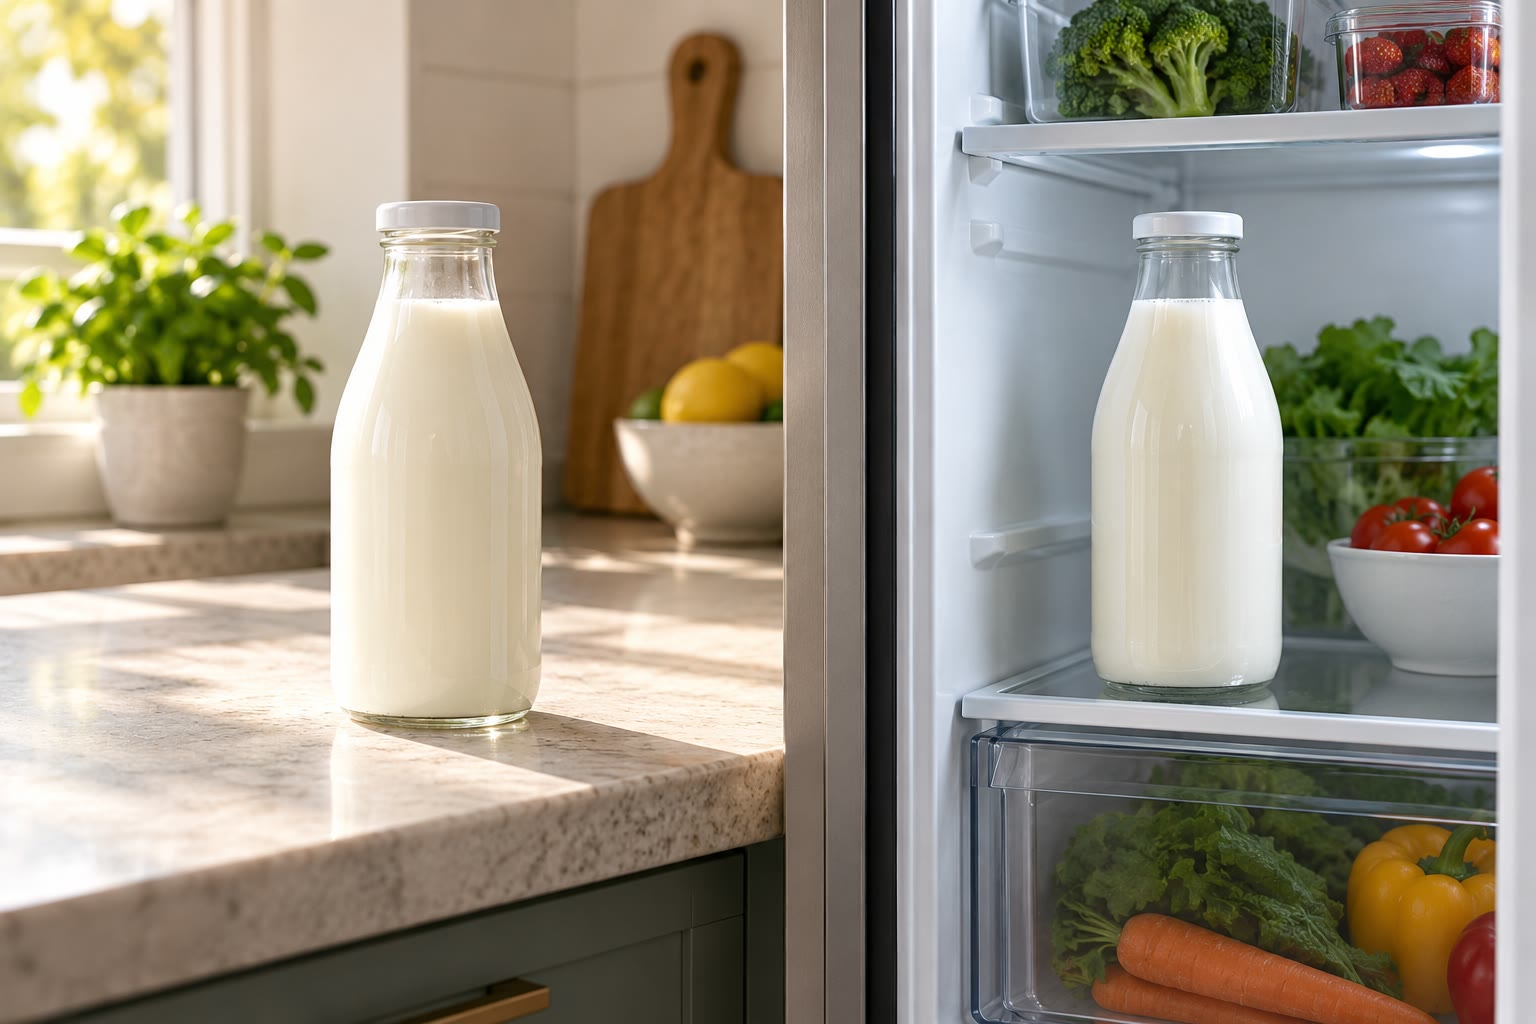
\includegraphics[width=0.48\linewidth]{images/book1/ai/g12-milk-counter-fridge.jpg}

{\small 同一瓶牛奶，分别放在台面与冰箱中：使它变酸的反应在低温下
更慢。}
\end{omfigure}

\section{随时间跟踪反应}

有些反应一旦\omterm{def:g7:chemical-reactions:reactant}{反应物}相遇便立即结束，例如氯化银的\omterm{def:g9:ions:precipitate}{沉淀反应}、酸与碱的反应。
另一些反应则需要数分钟、数小时甚至数年。
为研究慢反应，化学家定时测量\omterm{def:g7:chemical-reactions:reactant}{反应物}或生成物的浓度。
他们可以
\begin{itemize}
  \item 取少量样品，在每份样品中终止反应，再进行\omterm{def:g11:titration:titration}{滴定}；
  \item 当\omterm{def:g7:chemical-reactions:reactant}{反应物}或生成物有颜色时，
        测量溶液的\omterm{def:g11:absorbance:absorbance}{吸光度}；
  \item 测量放出气体的压强或体积，
        或\omterm{def:g9:ions:ion}{离子}发生变化的溶液的电导率。
\end{itemize}

\begin{definition}[淬灭]\label{def:g12:reaction-rates:quenching}
\emph{淬灭}\index{淬灭}样品，是指在取样时刻
使其中的反应停止或大大减慢，
通常的做法是骤然冷却并加以\omterm{def:g10:concentration-and-dilution:dilution}{稀释}，
以便从容地测定其组成。
\end{definition}

\begin{inthelab}[淬灭样品]
每隔五分钟，用移液管量取 \qty{10.0}{mL} 反应\omterm{def:g6:pure-substances-and-mixtures:mixture}{混合物}，
倒入盛有约 \qty{40}{mL} 冰水的烧杯中。
样品\omterm{def:g10:concentration-and-dilution:dilution}{稀释}为原来的五倍，并冷却至接近
\qty{0}{\celsius}，反应变得非常缓慢，可以认为已经停止；
随后对样品进行\omterm{def:g11:titration:titration}{滴定}。样品的时刻是将其倒入冰水的时刻，
而不是\omterm{def:g11:titration:titration}{滴定}的时刻。
\end{inthelab}

\begin{omfigure}
\begin{tikzpicture}[font=\small, scale=0.8]
  \pic[transform shape] at (0,0) {erlenmeyer={0.4}{orange!25}};
  \node[anchor=north, align=center] at (0,-0.15) {反应 \\ 混合物};
  \pic[transform shape, rotate=-35] at (1.4,1.2) {pipette={0.6}{orange!25}};
  \draw[omProp, very thick, -{Stealth}] (1.6,0.8) -- (2.9,0.8);
  \node[anchor=south] at (2.25,0.85) {\qty{10.0}{mL}};
  \pic[transform shape] at (4,0) {beaker={0.55}{cyan!12}};
  \foreach \p in {(3.6,0.4),(4.2,0.6),(3.9,0.85),(4.4,0.3)}
    \draw[black!30, fill=white] \p ++(-0.1,-0.08) rectangle ++(0.2,0.16);
  \node[anchor=north, align=center] at (4,-0.15) {冰水：\\ 反应终止};
  \draw[omProp, very thick, -{Stealth}] (5.1,0.8) -- (6.4,0.8);
  \pic[transform shape] at (7.5,0) {erlenmeyer={0.35}{orange!12}};
  \pic[transform shape] at (7.5,2.75) {burette={0.7}{violet!45}};
  \node[anchor=north, align=center] at (7.5,-0.15) {滴定 \\ 样品};
\end{tikzpicture}

{\small 通过取样跟踪反应：取出样品，\omterm{def:g12:reaction-rates:quenching}{淬灭}后
从容测定。}
\end{omfigure}

\section{动力学因素}

\begin{definition}[动力学因素]\label{def:g12:reaction-rates:kinetic-factor}
\emph{动力学因素}\index{动力学因素}是指能改变反应速率、
而不改变反应所得的产物：温度、
\omterm{def:g7:chemical-reactions:reactant}{反应物}的浓度、不同相\omterm{def:g7:chemical-reactions:reactant}{反应物}之间的接触面积，
以及催化剂的存在
（见下一章）。
\end{definition}

\begin{proposition}[温度越高、浓度越大、颗粒越细，反应越快]\label{prop:g12:reaction-rates:factors}
一般而言，温度越高、\omterm{def:g7:chemical-reactions:reactant}{反应物}越浓，
反应速率越快；对于固体\omterm{def:g7:chemical-reactions:reactant}{反应物}，
其越细碎，反应越快。
\end{proposition}

\begin{proof}
在本阶段不加证明地承认，附图示意：反应粒子必须相遇，
且相遇时要足够剧烈。增大浓度使相遇更频繁；将固体
分得更细则提供更多可以相遇的表面；升温使粒子运动加快，
从而相遇更频繁，尤其是使更多的相遇具有足以
断裂化学键的能量。
\end{proof}

\begin{example}[三个日常情形]\label{ex:g12:reaction-rates:everyday}
食物在冰箱中保存得更久，在冷冻室中则保存得久得多：
使食物变质的反应在低温下减慢。磨坊\omterm{def:g4:air-a-mixture-of-gases:air}{空气}中的细面粉尘
可能爆炸，而一袋面粉却只会阴燃：反应相同，
但接触面积大得多。能在水中起泡\omterm{def:g2:mixing-and-dissolving:dissolve}{溶解}的药片，
若先压碎，则\omterm{def:g2:mixing-and-dissolving:dissolve}{溶解}得更快。
\end{example}

\begin{omfigure}
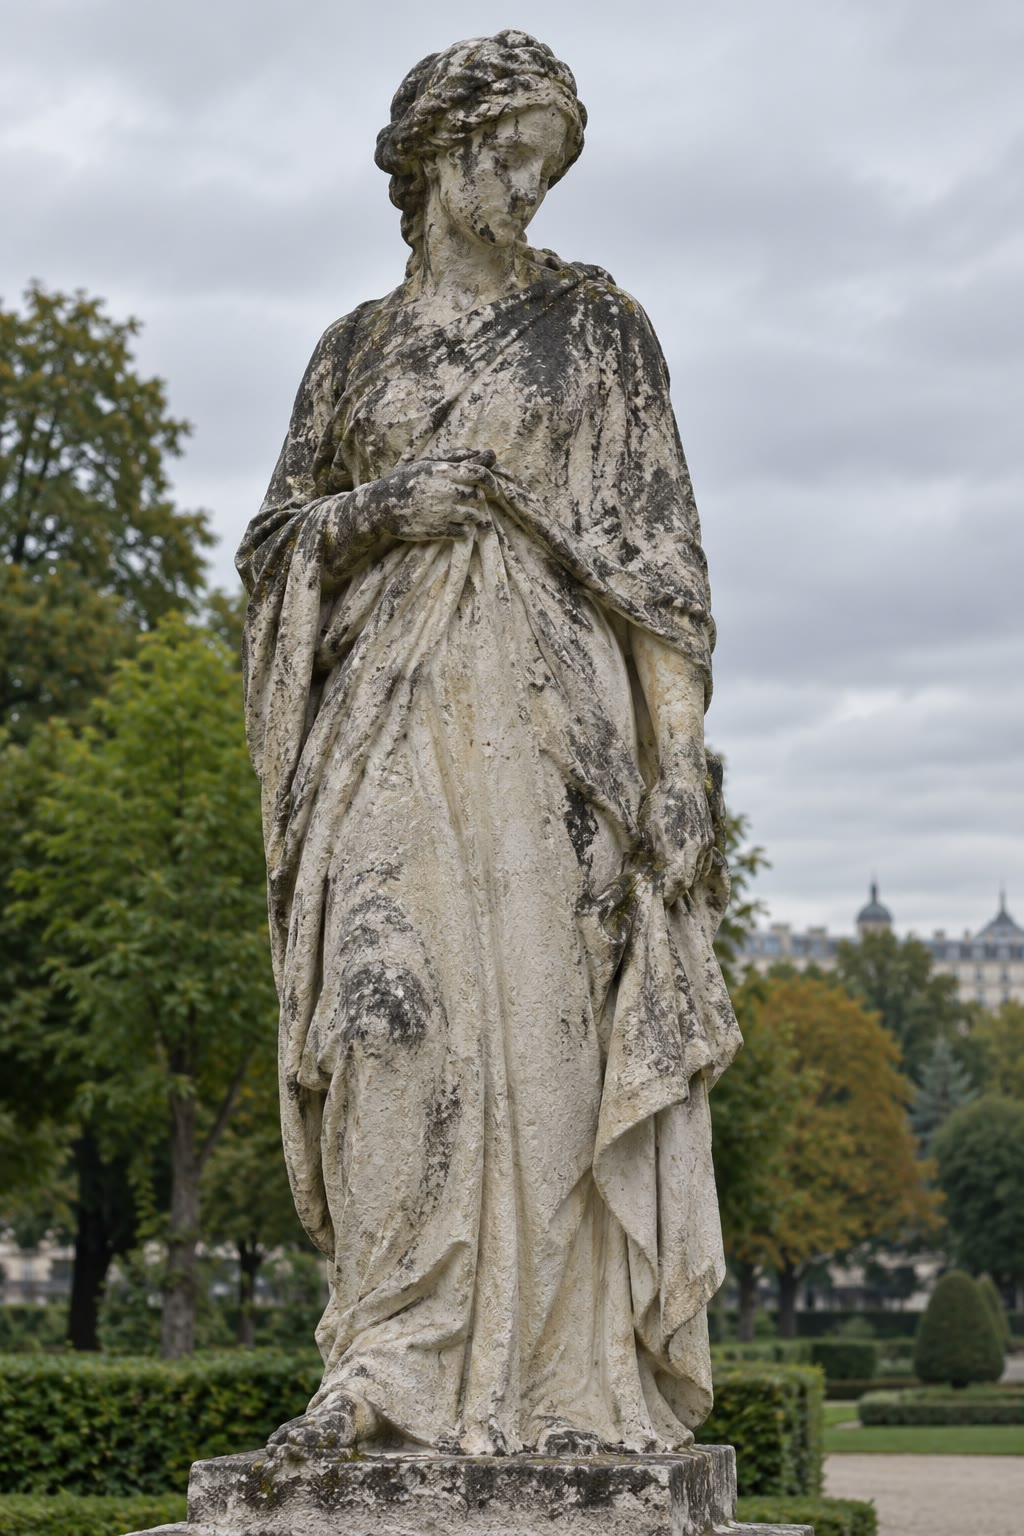
\includegraphics[width=0.42\linewidth,height=6cm,keepaspectratio]{images/book1/ai/g12-weathered-statue.jpg}

{\small 一座被雨水风化的石灰岩雕像：一个
历时数世纪的反应。}
\end{omfigure}

\section{消耗速率与生成速率}

\begin{definition}[消耗速率、生成速率]\label{def:g12:reaction-rates:rate}
在体积恒定的溶液中，\omterm{def:g7:chemical-reactions:reactant}{反应物} A 的\emph{消耗速率}\index{消耗速率}
在时刻 $t$ 时为
\[
  v_A(t) = -\frac{d[\ce{A}]}{dt},
\]
而生成物 P 的\emph{生成速率}\index{生成速率}
为 $v_P(t) = \dfrac{d[\ce{P}]}{dt}$，二者均为正，单位为
\si{mol.L^{-1}.min^{-1}}（或每秒）。
\end{definition}


\begin{method}[由切线读取速率]\label{met:g12:reaction-rates:tangent}
\begin{enumerate}
  \item 在 $[\ce{A}]$ 关于 $t$ 的曲线上，作
        所选时刻的切线。
  \item 在切线上取相距较远的两点，计算其斜率，
        即 $\Delta[\ce{A}] / \Delta t$。
  \item \omterm{def:g12:reaction-rates:rate}{消耗速率}等于该斜率的相反数（对于
        生成物，则为斜率本身）。
\end{enumerate}
\end{method}

\begin{omfigure}
\begin{tikzpicture}
\begin{axis}[width=0.8\linewidth, height=6.4cm, xmin=0, xmax=60, ymin=0,
    ymax=11, xlabel={$t$ (\si{min})}, ylabel={$[\ce{A}]$ (\si{mmol/L})},
    axis lines*=left, ymajorgrids, xmajorgrids, grid style={gray!20},
    tick label style={font=\small}, label style={font=\small},
    legend style={font=\small, at={(0.98,0.97)}, anchor=north east,
    draw=none, fill=white}, legend cell align=left]
  \addplot[very thick, omDef] table[x=t, y=A1] {figdata/out/grade-12-reaction-rates-a.dat};
  \addplot[very thick, omThm] table[x=t, y=A2] {figdata/out/grade-12-reaction-rates-a.dat};
  \addplot[thick, dashed, omProp, restrict y to domain=0:11] table[x=t, y=tangent]
    {figdata/out/grade-12-reaction-rates-a.dat};
  \legend{$k = \qty{0.050}{min^{-1}}$，$k = \qty{0.100}{min^{-1}}$（温度较高），
    $t = 0$ 处的切线}
  \addplot[densely dotted, black!60] coordinates {(0,5) (13.86,5) (13.86,0)};
  \addplot[densely dotted, black!60] coordinates {(6.93,5) (6.93,0)};
  \node[font=\small, anchor=south west] at (axis cs:14.6,5.4) {$t_{1/2} = \qty{13.9}{min}$};
  \node[font=\small, anchor=south east] at (axis cs:6.7,0.2) {\qty{6.9}{min}};
\end{axis}
\end{tikzpicture}

{\small 同一\omterm{def:g12:reaction-rates:first-order}{一级反应}在两种温度下，\omterm{def:g7:chemical-reactions:reactant}{反应物} A 的浓度随时间的变化。
$t = 0$ 处的切线（虚线）给出初始速率；
点线标出\omterm{def:g12:reaction-rates:half-life}{半衰期}。}
\end{omfigure}

\begin{example}[初始速率]\label{ex:g12:reaction-rates:initial}
在蓝色曲线上，$t = 0$ 处的切线
自 $t = 0$ 时的 \qty{10.0}{mmol/L} 降为 $0$（$t = \qty{20}{min}$ 时），其斜率为
$-10.0/20 = \qty{-0.50}{mmol.L^{-1}.min^{-1}}$，故初始\omterm{def:g12:reaction-rates:rate}{消耗速率}为
\qty{0.50}{mmol.L^{-1}.min^{-1}}。随后曲线趋于平缓，
速率下降：反应随着 A 的消耗而变慢。
\end{example}

\section{一级反应}

\begin{definition}[一级反应、速率常数]\label{def:g12:reaction-rates:first-order}
若某反应对 A 为\emph{一级反应}\index{一级反应}，
即 A 的\omterm{def:g12:reaction-rates:rate}{消耗速率}
在每一时刻都与 A 的浓度成正比：
\[
  -\frac{d[\ce{A}]}{dt} = k\,[\ce{A}] .
\]
正常数 $k$，单位为 \si{min^{-1}} 或 \si{s^{-1}}，是
\emph{速率常数}\index{速率常数}；它依赖于温度。
\end{definition}

\begin{proposition}[指数衰减]\label{prop:g12:reaction-rates:exponential}
对于初始浓度为 $[\ce{A}]_0$ 的\omterm{def:g12:reaction-rates:first-order}{一级反应}，
\[
  [\ce{A}](t) = [\ce{A}]_0\, e^{-kt} .
\]
\end{proposition}

\begin{proof}
函数 $f(t) = [\ce{A}]_0 e^{-kt}$ 的导数为
$f'(t) = -k [\ce{A}]_0 e^{-kt} = -k f(t)$，故它满足速率方程，
且 $f(0) = [\ce{A}]_0$。它是满足此条件的唯一函数，
这一点在本阶段不加证明地承认（该结论在数学中对 $y' = ay$ 的方程给出证明）。
\end{proof}

\begin{method}[检验是否为一级反应]\label{met:g12:reaction-rates:test}
\begin{enumerate}
  \item 由测量数据，计算各时刻的 $\ln [\ce{A}]$
        代以 $\ln A$（\omterm{def:g11:absorbance:absorbance}{吸光度}正比于 $[\ce{A}]$）。
  \item 作 $\ln[\ce{A}]$ 关于 $t$ 的图像。由于
        $\ln[\ce{A}] = \ln[\ce{A}]_0 - kt$，各点落在一条直线上，
        当且仅当该反应为\omterm{def:g12:reaction-rates:first-order}{一级反应}。
  \item 直线的斜率为 $-k$。
\end{enumerate}
\end{method}

\section{半衰期}

\begin{definition}[半衰期]\label{def:g12:reaction-rates:half-life}
反应的\emph{半衰期}\index{半衰期} $t_{1/2}$ 是指
\omterm{def:g10:reaction-progress-table:limiting}{限量反应物}的浓度降至初始值的一半
所需的时间。
\end{definition}

\begin{proposition}[一级反应的半衰期]\label{prop:g12:reaction-rates:half-life}
对于\omterm{def:g12:reaction-rates:first-order}{一级反应}，
\[
  t_{1/2} = \frac{\ln 2}{k},
\]
与初始浓度无关；经过 $n$ 个\omterm{def:g12:reaction-rates:half-life}{半衰期}后，
浓度被除以 $2^n$。
\end{proposition}

\begin{proof}
$[\ce{A}]_0 e^{-k t_{1/2}} = [\ce{A}]_0 / 2$ 可得 $e^{-k t_{1/2}} = 1/2$，
于是 $k t_{1/2} = \ln 2$。每经过一个\omterm{def:g12:reaction-rates:half-life}{半衰期}，
浓度就再乘以 $e^{-k t_{1/2}} = 1/2$。
\end{proof}


\begin{example}[读取半衰期]\label{ex:g12:reaction-rates:half-lives}
当 $k = \qty{0.050}{min^{-1}}$ 时，$t_{1/2} = 0.693 / 0.050 =
\qty{13.9}{min}$：浓度由 10.0 降至 5.0，再降至 2.5，
又降至 \qty{1.25}{mmol/L}，对应时刻依次为 13.9、27.7 和 \qty{41.6}{min}。温度较高的一组，
$k$ 为原来的两倍，\omterm{def:g12:reaction-rates:half-life}{半衰期}减半，为 \qty{6.9}{min}，
如图所示。
\end{example}

\begin{remark}[其他场合的半衰期]\label{rem:g12:reaction-rates:radioactive}
物理学中同一术语也用于放射性\omterm{def:g9:inside-the-atom:nucleus}{原子核}，其数目
同样按指数规律减少：放射性衰变的行为类似于
\omterm{def:g12:reaction-rates:first-order}{一级反应}。这一内容在物理学分册中有所讨论。
\end{remark}

\begin{omfigure}
\begin{minipage}{0.49\linewidth}
\begin{tikzpicture}
\begin{axis}[width=\linewidth, height=5.4cm, xmin=0, xmax=26, ymin=0,
    ymax=0.85, xlabel={$t$ (\si{min})}, ylabel={吸光度 $A$},
    axis lines*=left, ymajorgrids, grid style={gray!20},
    tick label style={font=\scriptsize}, label style={font=\small}]
  \addplot[only marks, mark=*, mark size=1.8pt, omDef] table[x=t, y=A]
    {figdata/out/grade-12-reaction-rates-b.dat};
  \addplot[thick, omProp, domain=0:26, samples=60] {0.8*exp(-0.11552*x)};
\end{axis}
\end{tikzpicture}
\end{minipage}\hfill
\begin{minipage}{0.49\linewidth}
\begin{tikzpicture}
\begin{axis}[width=\linewidth, height=5.4cm, xmin=0, xmax=26, ymin=-3.4,
    ymax=0, xlabel={$t$ (\si{min})}, ylabel={$\ln A$}, axis lines*=left,
    ymajorgrids, grid style={gray!20}, tick label style={font=\scriptsize},
    label style={font=\small}]
  \addplot[only marks, mark=*, mark size=1.8pt, omDef] table[x=t, y=lnA]
    {figdata/out/grade-12-reaction-rates-b.dat};
  \addplot[thick, omProp, domain=0:26] {-0.2231-0.11552*x};
\end{axis}
\end{tikzpicture}
\end{minipage}

{\small \omterm{def:g9:acids-bases-ph:acidic}{碱性溶液}中结晶紫的褪色（取自
周末问题的数据）。左图：\omterm{def:g11:absorbance:absorbance}{吸光度}沿指数曲线下降。
右：$\ln A$ 对 $t$ 的图像是一条直线，斜率为
$-\qty{0.116}{min^{-1}}$，表明该反应对染料为一级。}
\end{omfigure}

\section{练习}

\begin{exercise}[$\star$]\label{exo:g12:reaction-rates:1}
指出下列各种情形中起作用的\omterm{def:g12:reaction-rates:kinetic-factor}{动力学因素}：冰箱可以保存食物；
粉状糖比块状糖\omterm{def:g2:mixing-and-dissolving:dissolve}{溶解}得快；浓度更高的酸
与锌反应更快；切开的苹果在夏天变褐更快。
\end{exercise}

\begin{exercise}[$\star$]\label{exo:g12:reaction-rates:2}
由 $[\ce{A}]$ 随时间变化的图像，读出每组实验的\omterm{def:g12:reaction-rates:half-life}{半衰期}。
蓝色曲线上，经过两个\omterm{def:g12:reaction-rates:half-life}{半衰期}后 $[\ce{A}]$ 为多少？
\end{exercise}

\begin{exercise}[$\star$]\label{exo:g12:reaction-rates:3}
过生成物曲线在 $t = \qty{5}{min}$ 处所作的切线，
经过 $(0, \qty{1.0}{mmol/L})$ 与 $(\qty{10}{min}, \qty{5.0}{mmol/L})$ 两点。
求 \qty{5}{min} 时生成物的\omterm{def:g12:reaction-rates:rate}{生成速率}。
\end{exercise}

\begin{exercise}[$\star$]\label{exo:g12:reaction-rates:4}
为什么\omterm{def:g11:titration:titration}{滴定}前要把试样倒入冰冷的水中？为什么
试样的时刻必须记在倒入之时，而不是
\omterm{def:g11:titration:titration}{滴定}之时？
\end{exercise}

\begin{exercise}[$\star$]\label{exo:g12:reaction-rates:5}
某\omterm{def:g12:reaction-rates:first-order}{一级反应}的\omterm{def:g12:reaction-rates:half-life}{半衰期}为 \qty{10}{min}。求\omterm{def:g7:chemical-reactions:reactant}{反应物}
经过 \qty{30}{min} 后剩余的分数；经过 \qty{1}{h} 后又是多少？
\end{exercise}

\begin{exercise}[$\star\star$]\label{exo:g12:reaction-rates:6}
\omterm{def:g7:chemical-reactions:reactant}{反应物}的浓度（单位 \si{mmol/L}）：在 \qty{0}{min} 时为 8.00，
在 \qty{5}{min} 时为 5.66，在 \qty{10}{min} 时为 4.00，在 \qty{15}{min} 时为 2.83，
在 \qty{20}{min} 时为 2.00。求各时刻的 $\ln[\ce{A}]$，
并证明反应为一级；求 $k$ 与\omterm{def:g12:reaction-rates:half-life}{半衰期}。
\end{exercise}

\begin{exercise}[$\star\star$]\label{exo:g12:reaction-rates:7}
\omterm{def:g12:reaction-rates:first-order}{一级反应}的 $t_{1/2} = \qty{25}{s}$。求 $k$。
\end{exercise}

\begin{exercise}[$\star\star$]\label{exo:g12:reaction-rates:8}
已知 $[\ce{A}]_0 = \qty{0.100}{mol/L}$，$k = \qty{0.020}{min^{-1}}$，
求经过 10、30 和 \qty{100}{min} 后的 $[\ce{A}]$。
\end{exercise}

\begin{exercise}[$\star\star$]\label{exo:g12:reaction-rates:9}
在 $[\ce{A}]$ 随时间变化的图上，估计蓝色
曲线在 $t = \qty{13.9}{min}$ 处的斜率（作切线），并与
该时刻的 $-k[\ce{A}]$ 比较。
\end{exercise}

\begin{exercise}[$\star\star$]\label{exo:g12:reaction-rates:10}
在无色溶液中，棕色的碘 \ce{I2} 缓慢生成。
\omterm{def:g11:absorbance:absorbance}{吸光度}由 0 逐渐升至 0.60。说明为何可用\omterm{def:g11:absorbance:absorbance}{吸光度}
来跟踪 $[\ce{I2}]$ 的变化，以及如何在
$A$ 对 $t$ 的曲线上读出某一时刻的\omterm{def:g12:reaction-rates:rate}{生成速率}。
\end{exercise}

\begin{exercise}[$\star\star$]\label{exo:g12:reaction-rates:11}
同一反应进行两组实验，起始时 $[\ce{A}]_0 = 10$ 与
\qty{20}{mmol/L}。若该反应为\omterm{def:g12:reaction-rates:first-order}{一级反应}，比较两者的初始
速率和\omterm{def:g12:reaction-rates:half-life}{半衰期}。
\end{exercise}

\begin{exercise}[$\star\star\star$]\label{exo:g12:reaction-rates:12}
\omterm{def:g12:reaction-rates:first-order}{一级反应}的\omterm{def:g7:chemical-reactions:reactant}{反应物}需经过多少个\omterm{def:g12:reaction-rates:half-life}{半衰期}，才降至
初始量的 \qty{1}{\percent}？\qty{0.1}{\percent} 呢？
给出降至分数 $f$ 所需时间的一般公式。
\end{exercise}

\begin{exercise}[$\star\star\star$]\label{exo:g12:reaction-rates:13}
某反应在 \qty{20}{\celsius} 时，$k = \qty{0.050}{min^{-1}}$，
在 \qty{30}{\celsius} 时 $k = \qty{0.100}{min^{-1}}$。两种温度下耗尽
\qty{90}{\percent} 的\omterm{def:g7:chemical-reactions:reactant}{反应物}各需多长时间？常用经验规则认为
温度每升高 \qty{10}{\celsius}，速率便加倍：
此反应是否遵循这一规则？
\end{exercise}

\begin{exercise}[$\star\star\star$]\label{exo:g12:reaction-rates:14}
将一份样品 \qty{5.0}{mL} 倒入 \qty{45}{mL} 冰水中以
\omterm{def:g12:reaction-rates:quenching}{淬灭}反应。给出反应明显变慢的两个原因。若该反应
对两种\omterm{def:g7:chemical-reactions:reactant}{反应物}各为一级，仅\omterm{def:g10:concentration-and-dilution:dilution}{稀释}作用使速率
除以的因子是多少？
\end{exercise}

\begin{exercise}[$\star\star\star$]\label{exo:g12:reaction-rates:15}
对\omterm{def:g12:reaction-rates:first-order}{一级反应}，求导证明其\omterm{def:g12:reaction-rates:rate}{消耗速率}
本身是时间的指数函数，
即 $v(t) = k[\ce{A}]_0 e^{-kt}$。初始速率是多少？经过多长时间，
速率恰为初始速率的一半？
\end{exercise}

\section{问题：褪色的染料}

\begin{problem}[{周末问题——结晶紫被氢氧根
离子漂白：颜色几乎褪尽需要多长时间？}]
\label{pb:g12:reaction-rates:1}
染料结晶紫与氢氧根\omterm{def:g9:ions:ion}{离子}反应，生成
无色产物。氢氧根大量过量时，速率
仅取决于染料的浓度。溶液的\omterm{def:g11:absorbance:absorbance}{吸光度}
在染料吸收最强的波长处记录：
\begin{center}
\small
\begin{tabular}{l*{10}{c}}
\hline
$t$ (\si{min}) & 0 & 2 & 4 & 6 & 8 & 10 & 12 & 15 & 20 & 25 \\
$A$ & 0.800 & 0.639 & 0.501 & 0.402 & 0.315 & 0.255 & 0.199 & 0.143 &
0.078 & 0.046 \\
\hline
\end{tabular}
\end{center}

\medskip
\noindent\textbf{第一部分——\omterm{def:g11:absorbance:absorbance}{吸光度}与浓度。}
\begin{enumerate}
  \item 为何\omterm{def:g11:absorbance:absorbance}{吸光度}与染料的
        浓度成正比？溶液须满足什么条件？
  \item 为何无色的产物在此波长下看不到？
  \item 为何氢氧根要大量过量？
  \item 反应结束时，分光光度计上
        应读到什么读数？
\end{enumerate}

\medskip
\noindent\textbf{第二部分——是否为\omterm{def:g12:reaction-rates:first-order}{一级反应}？}
\begin{enumerate}[resume]
  \item 直接从表中读出\omterm{def:g12:reaction-rates:half-life}{半衰期}。
  \item 检验 $t = 6$ 至 $t = 12$ 分钟之间的\omterm{def:g12:reaction-rates:half-life}{半衰期}是否不变。
  \item 计算各时刻的 $\ln A$。
  \item 作 $\ln A$ 对 $t$ 的图（或利用本章的图）。观察到
        什么现象？由此得出结论。
  \item 由 0 与 \qty{20}{min} 两点处的数据计算斜率。
\end{enumerate}

\medskip
\noindent\textbf{第三部分——\omterm{def:g12:reaction-rates:first-order}{速率常数}。}
\begin{enumerate}[resume]
  \item 求出 $k$。
  \item 由 $k$ 计算\omterm{def:g12:reaction-rates:half-life}{半衰期}，并与第 5 题的结果比较。
  \item 计算染料的初始\omterm{def:g12:reaction-rates:rate}{消耗速率}，
        以\omterm{def:g11:absorbance:absorbance}{吸光度}的下降速率表示。
  \item 若初始\omterm{def:g11:absorbance:absorbance}{吸光度}为 0.400，\omterm{def:g12:reaction-rates:half-life}{半衰期}将为多少？
\end{enumerate}

\medskip
\noindent\textbf{第四部分——预测。}
\begin{enumerate}[resume]
  \item 预测在 \qty{30}{min} 时的\omterm{def:g11:absorbance:absorbance}{吸光度}。
  \item \omterm{def:g11:absorbance:absorbance}{吸光度}于何时降至 0.008，即
        起始值的 \qty{1}{\percent}？
  \item 这相当于多少个\omterm{def:g12:reaction-rates:half-life}{半衰期}？
  \item \omterm{def:g11:absorbance:absorbance}{吸光度}低于约 $A = 0.010$ 时，人眼
        便不再看到颜色。溶液何时看起来无色？
  \item 将实验在高出 \qty{10}{\celsius} 的温度下重复，
        \omterm{def:g12:reaction-rates:half-life}{半衰期}变为 \qty{3.0}{min}。何时
        达到 \qty{1}{\percent}？
  \item 给出最终结论：颜色降至起始值的
        \qty{1}{\percent} 需要经过多少个\omterm{def:g12:reaction-rates:half-life}{半衰期}，
        这在本题中对应多少分钟？
\end{enumerate}
\end{problem}
